\documentclass{ctexart}
\usepackage{Note}
\begin{document}
\section{图像处理}
\subsection{图像的表示方法}
图像在本质上是连续的图形,但计算机并不能存储无限的信息,因此需要对图像进行离散化处理.
\begin{definition}[位图与矢量图]
    位图(Bitmap)是由像素点组成的矩阵,每个像素点有一个颜色值,通过这些像素点的颜色值来表示图像.
    矢量图(Vector Graphics)是由数学方程和几何图形(如直线,曲线,多边形等)来表示图像.
\end{definition}
两者之间的差异可以由下表总结:
\begin{table}[h]
    \centering
    \begin{tabular}{ccc}
        \hline
        & 位图 & 矢量图 \\
        \hline
        优点 & 可以表示复杂的图像细节 & 可以无限放大而不失真 \\
        \hline
        缺点 & 放大后会失真 & 难以表示复杂的图像细节 \\
        \hline
    \end{tabular}
    \caption{位图与矢量图的比较}
\end{table}
\subsection{Fourier变换与图像的频谱}
\subsubsection{Fourier级数的复变函数形式}
在高等数学中,对周期为$T$的函数$f(x)$的Fourier级数展开为
\[f(x)=\dfrac{a_0}{2}+\sum_{n=1}^{\infty}\left[a_n\cos\left(\dfrac{2n\pi x}{T}\right)+b_n\sin\left(\dfrac{2n\pi x}{T}\right)\right]\]
其中
\[a_0=\dfrac{2}{T}\int_{-T/2}^{T/2}f(x)\di x,\ \ a_n=\dfrac{2}{T}\int_{-T/2}^{T/2}f(x)\cos\left(\dfrac{2n\pi x}{T}\right)\di x,\ \ b_n=\dfrac{2}{T}\int_{-T/2}^{T/2}f(x)\sin\left(\dfrac{2n\pi x}{T}\right)\di x\]
\indent 考虑到复平面圆周与简谐波的关系(这也方便各种变换与数学处理),我们尝试把上面的式子改写成复变函数的形式.由Euler公式
\[\e^{\i\theta}=\cos\theta+\i\sin\theta\]
可得
\[\cos\theta=\dfrac{\e^{\i\theta}+\e^{-\i\theta}}{2},\ \ \sin\theta=\dfrac{\e^{\i\theta}-\e^{-\i\theta}}{2\i}\]
令$\omega=\dfrac{2\pi}{T}$,于是
\[\begin{aligned}
    f(x)
    &= \dfrac{a_0}{2}+\sum_{n=1}^{\infty}\left[a_n\cos(n\omega x)+b_n\sin(n\omega x)\right]\\
    &= \dfrac{a_0}{2}+\sum_{n=1}^{\infty}\left(a_n\dfrac{\e^{\i n\omega x}+\e^{-\i n\omega x}}{2}+b_n\dfrac{\e^{\i n\omega x}-\e^{-\i n\omega x}}{2\i}\right)\\
    &= \dfrac{a_0}{2}+\sum_{n=1}^{\infty}\left(\dfrac{a_n-\i b_n}{2}\e^{\i n\omega x}+\dfrac{a_n+\i b_n}{2}\e^{-\i n\omega x}\right)
\end{aligned}\]
为了将求和的两部分统一起来,注意到
\[a_{-n}=\dfrac{2}{T}\int_{-T/2}^{T/2}f(x)\cos\left(\dfrac{-2n\pi x}{T}\right)\di x=a_n\]
\[b_{-n}=\dfrac{2}{T}\int_{-T/2}^{T/2}f(x)\sin\left(-\dfrac{2n\pi x}{T}\right)\di x=-b_n\]
于是上式可以改写为
\[f(x)
=\dfrac{a_0}{2}+\sum_{n=1}^{\infty}\dfrac{a_n-\i b_n}{2}\e^{\i n\omega x}+\sum_{n=1}^{\infty}\dfrac{a_{-n}-\i b_{-n}}{2}\e^{\i(-n)\omega x}
=\sum_{n=-\infty}^{\infty}\dfrac{a_n-\i b_n}{2}\e^{\i n\omega x}\]
定义$C_n=\dfrac{a_n-\i b_n}{2}$,就可以得到Fourier级数写成复变函数的形式:
\[f(x)=\sum_{n=-\infty}^{\infty}C_n\e^{\i n\omega x}\]
现在,我们考虑系数$C_n$的求法.我们在上述展开式两边乘以$\e^{-\i m\omega x}$,然后在一个周期(例如$[0,T]$)上积分,就有
\[\int_{0}^{T}f(x)\e^{-\i m\omega x}\di x
=\int_{0}^{T}\left(\sum_{n=-\infty}^{+\infty}C_n\e^{\i(n-m)\omega x}\right)\di x
=\sum_{n=-\infty}^{+\infty}C_n\int_{0}^{T}\e^{\i(n-m)\omega x}\di x\]
当$n=m$时,上面右边的积分值为$T$,否则令$k=n-m$就有
\[\int_0^{T}\e^{\i(n-m)\omega x}\di x=\int_0^{T}\exp\left(\dfrac{2\pi\i kx}{T}\right)\di x=\dfrac{T\left(\e^{2k\pi\i}-1\right)}{2\pi\i k}=0\]
于是
\[\int_{0}^{T}f(x)\e^{-\i m\omega x}\di x=TC_m\]
这样就有
\[C_n=\dfrac{1}{T}\int_{0}^{T}f(x)\e^{-\i n\omega x}\di x\]
\begin{theorem}[Fourier级数展开的复变函数形式]
    设$f(x)$为周期为$T$的满足Dirichlet条件的函数,则$f(x)$可以展开为Fourier级数
    \[f(x)=\sum_{n=-\infty}^{\infty}C_n\e^{\i n\omega x}\]
    其中$\omega=\dfrac{2\pi}{T}$,系数$C_n$由下式给出:
    \[C_n=\dfrac{1}{T}\int_{0}^{T}f(x)\e^{-\i n\omega x}\di x\]
\end{theorem}
\subsubsection{从Fourier级数到Fourier变换}
那么对于非周期函数,我们可以将其视作周期$T\to+\infty$的周期函数,此时角频率$\dfrac{2\pi}{T}\to0$, Fourier级数中的$n\omega$也应当取遍任意实数.因此,将Fourier展开中的求和变成积分,并且将系数$C_n$换成有关$\omega$的函数$F(\omega)$,即
\[f(x)=\int_{-\infty}^{+\infty}F(\omega)\e^{\i \omega x}\di\omega\]
同样地,每个$\omega$对应的系数$F(\omega)$也可以由$f(x)$求出,即
\[F(\omega)=\dfrac{1}{2\pi}\int_{-\infty}^{+\infty}f(x)\e^{-\i \omega x}\di x\]
在很多场合下,通常令$f=\dfrac{\omega}{2\pi}=\dfrac{1}{T}$为频率(更经常地, $f$也被记作$\omega$,注意与前面推导中的角频率加以区分),这就得到Fourier变换的标准形式.同时,我们在后面附上一个比较严谨的证明.
\begin{theorem}
    设$f(x)$满足Fourier变换的条件,则$f(x)$的Fourier变换为
    \[F(\omega)=\mathcal{F}\circ f=\int_{-\infty}^{+\infty}f(x)\e^{-2\pi\i\omega x}\di x\]
    其逆变换为
    \[f(x)=\mathcal{F}^{-1}\circ F=\int_{-\infty}^{+\infty}F(\omega)\e^{2\pi\i\omega x}\di\omega\]
\end{theorem}
\begin{proof}
    证明中的$\omega$采取我们后来给出的定义.由Fourier级数展开的复变函数形式,对于周期为$T$的函数$f(x)$,有
    \[f(x)=\sum_{n=-\infty}^{+\infty}C_n\e^{2\pi\i n\omega x}=\sum_{n=-\infty}^{+\infty}\dfrac{C_n}{\omega}\left(\omega\e^{2\pi\i n\omega x}\right)\]
    其中$\omega=1/T$而
    \[\dfrac{C_n}{\omega}=\dfrac{1}{\omega}\cdot\dfrac{1}{T}\int_0^{T}f(x)\e^{-2\pi\i n\omega x}\di x=\int_{-T/2}^{T/2}f(x)\e^{-2\pi\i n\omega x}\di x\]
    现在令$T\to\infty$,于是$\omega=1/T\to0$.现在令$t=n\omega$,于是
    \[\begin{aligned}
        f(x)
        &= \lim_{\omega\to0}\sum_{n=-\infty}^{+\infty}\dfrac{C_n}{\omega}\left(\omega\e^{2\pi\i n\omega x}\right) \\
        &= \lim_{\omega\to0}\sum_{n=-\infty}^{+\infty}\omega\e^{2\pi\i n\omega x}\left(\int_{-T/2}^{T/2}f(x)\e^{-2\pi\i n\omega x}\di x\right) \\
        &= \lim_{\omega\to0}\sum_{n=-\infty}^{+\infty}\e^{2\pi\i t x}\left(\int_{-\infty}^{+\infty}f(x)\e^{-2\pi\i t x}\di x\right)\omega\\
    \end{aligned}\]
    上面的求和与Riemann积分的定义一致,因此
    \[f(x)=\int_{-\infty}^{+\infty}\e^{2\pi\i t x}\left(\int_{-\infty}^{+\infty}f(x)\e^{-2\pi\i t x}\di x\right)\di t\]
    把$t$换成$\omega$,将中间的积分记作$F(\omega)$,即可证得定理.
\end{proof}
\subsubsection{离散信号的Fourier变换}
对于无限长度的离散信号$\{x[n]\}_{n\in\mathcal{Z}}$,我们可以把无穷积分换成无穷级数求和.记其Fourier变换的结果为$\hat{x}(\omega)$,则
\[\hat{x}(\omega)=\sum_{n=-\infty}^{+\infty}x[n]\e^{-2\pi\i\omega n}\]
\indent 然而,计算机存储的信号数目是有限的.因此,对于一段有限长度为$N$的离散信号$\{x[n]\}_{0\leqslant n< N}$,我们假设它可以周期延拓(相当于$\{x[n]\}$是周期为$N$的函数的$N$个采样点),这时的Fourier变换即Fourier展开,频率的选取是离散的;并且由于我们只有$N$个数据点,因此最多只有$N$个独立的频率对应的简谐波合成了这一离散信号.于是
\[\hat{x}[k]=\sum_{n=0}^{N-1}\exp\left(-\dfrac{2\pi\i nk}{N}\right)x[n],\ \ k=0,1,\cdots,N-1\]
它的逆变换为
\[x[n]=\dfrac{1}{N}\sum_{k=0}\exp\left(\dfrac{2\pi\i nk}{N}\right)\hat{x}[k]\]
同样地,二维情形下的Fourier变换为
\[F(u,v)=\int_{-\infty}^{+\infty}\int_{-\infty}^{+\infty}f(x,y)\e^{-2\pi\i(ux+vy)}\di x\di y\]
其中$\e^{-2\pi\i(ux+vy)}$表示方向向量为$(u,v)$,频率为$\sqrt{u^2+v^2}$的复平面上的波(同样地由正弦波和余弦波组成).也同样地,离散情形下的二维Fourier变换为
\[\hat{\mat{I}}(u,v)=\sum_{x=0}^{M-1}\sum_{y=0}^{N-1}\mat{I}(x,y)\exp\left[-2\pi\i\left(\dfrac{ux}{M}+\dfrac{vy}{N}\right)\right],\ \ 0\leqslant u<M,0\leqslant v<N\]
于是$\hat{\mat{I}}(u,v)$也是一个$M\times N$的矩阵,这就是$\mat{I}$的频谱.对频谱$\hat{\mat{I}}$做逆Fourier变换可以还原出图像$\mat{I}$.
\subsection{图像滤波}
\subsubsection{卷积}
卷积是图像处理中常用的操作,用于图像的平滑,锐化,边缘检测等.
\begin{definition}[卷积]
    二维离散信号(如图像)的卷积定义为:
    \[
        (\mat{I} * \mat{K})(x,y) = \sum_{m=-M}^{M} \sum_{n=-N}^{N} \mat{I}(x-m,y-n)\mat{K}(m,n)
    \]
    其中$\mat{I}$是输入图像, $\mat{K}$是卷积核(滤波器),$(x,y)$是图像中的一个像素位置.在图形学的实际应用中,卷积核通常经过预翻转操作,此时卷积定义为
    \[(\mat{I} * \mat{K})(x,y) = \sum_{m=-M}^{M} \sum_{n=-N}^{N} \mat{I}(x+m,y+n)\mat{K}(m,n)\]
\end{definition}
卷积和傅里叶变换密切相关.
\begin{theorem}[卷积定理]
    函数卷积的傅里叶变换等于各自傅里叶变换的乘积,即
    \[\mathcal{F}(f * g) = \mathcal{F}(f) \cdot \mathcal{F}(g)\]
\end{theorem}
这样,可以观察图像和滤波器进行傅里叶变换的频谱来大致得出滤波后的结果,从而针对性地设计滤波器.
\subsubsection{图像模糊}
最简单的模糊滤波器是均值滤波器.
\begin{definition}[均值滤波器]
    均值滤波器的卷积核为
    \[\mat{K}_{\text{mean}}=\dfrac{1}{(2k+1)^2}\begin{bmatrix}
        1&\cdots&1\\
        \vdots&\ddots&\vdots\\
        1&\cdots&1
    \end{bmatrix}\]
\end{definition}
根据卷积的定义,均值滤波器的作用是取目标像素邻近的$(2k+1)\times(2k+1)$个像素求平均值.\\
\indent 均值滤波器地频谱主要集中在低频部分,可以去除高频噪声,但会模糊图像细节.然而,它的频谱有呈十字形向外放射的部分,因此使用均值滤波器可能导致细节错误.\\
\indent 高斯滤波器是一种效果更好的模糊滤波器\footnote{在Adobe Photoshop中对应高斯模糊选项.}.它的连续形式为
\[g(x,y)=\dfrac{1}{2\pi\sigma^2}\exp\left(-\dfrac{x^2+y^2}{2\sigma^2}\right)\]
其中$\sigma$为方差,可以控制模糊程度.实际使用时,可以截取目标附近的$(2k+1)\times(2k+1)$个像素,根据上述函数计算权重并归一化得到卷积核,然后按照类似均值滤波的计算方式完成卷积.\\
\indent 在数学上可以证明,高斯滤波器的频谱仍然是高斯函数,只保留低频部分,不会出现像均值滤波器那样的走样.
\subsubsection{边缘提取}
所谓图像中的边缘,是指图像中一个色块与另一个色块的分界线,通常对应图像中颜色变化较大的部分.我们可以用估计梯度的算子来提取边缘.
\begin{definition}[Sobel算子]
    Sobel算子是一种常用的边缘检测算子,它通过两个卷积核来计算图像在水平和垂直方向上的梯度:
    \[
        \mat{K}_x = \begin{bmatrix}
            -1 & 0 & 1 \\
            -2 & 0 & 2 \\
            -1 & 0 & 1
        \end{bmatrix},\quad
        \mat{K}_y = \begin{bmatrix}
            1 & 2 & 1 \\
            0 & 0 & 0 \\
            -1 & -2 & -1
        \end{bmatrix}
    \]
    其中$\mat{K}_x$用于检测水平边缘, $\mat{K}_y$用于检测垂直边缘.\\
    对图像$\mat{I}$进行卷积后,可以得到水平和垂直方向的梯度:
    \[
        G_x = \mat{I} * \mat{K}_x,\quad G_y = \mat{I} * \mat{K}_y
    \]
    为了得出各个方向上的边缘,可以计算指定位置的梯度向量的模长:
    \[
        G = \sqrt{G_x^2 + G_y^2}
    \]
\end{definition}
除了使用梯度提取边缘,还可以使用二阶导数提取边缘.
\begin{definition}[Laplacian算子]
    Laplacian算子是一种二阶导数算子,用于检测图像中的边缘.其卷积核为
    \[
        \mat{K}_{\text{Lap}} = \begin{bmatrix}
            0 & 1 & 0 \\
            1 & -4 & 1 \\
            0 & 1 & 0
        \end{bmatrix}
    \]
    对图像$\mat{I}$进行卷积后,可以得到Laplacian响应:
    \[L = \mat{I} * \mat{K}_{\text{Lap}}\]
    Laplacian算子对噪声较敏感,因此通常在使用前先对图像进行高斯模糊处理,这种方法称为LoG(Laplacian of Gaussian).
\end{definition}
\subsection{图像补全与融合}
在图像补全时,我们需要对图像缺失的部分进行补充,并且使得结果看起来更为自然,即满足下面两个条件:
\begin{enumerate}[label=\tbf{\arabic*.},topsep=0pt,parsep=0pt,itemsep=0pt,partopsep=0pt]
    \item \tbf{空间局部性}:同一个物体上相邻的部分应当相似.
    \item \tbf{奥卡姆剃刀原理}:如无必要,勿增实体.
\end{enumerate}
\indent 在数学上,我们可以用以下的办法描述问题:考虑图像$I$的待补全区域$\Omega$以及其边界$\partial \Omega$.定义$f(x,y)$为$\Omega\cup\p\Omega$上的函数表示待填补的颜色, $f^\ast(x,y)$为$\complement_I\Omega$上的函数表示已知的颜色.于是优化目标为
\[\min_f\iint_{\Omega}\left|\left|\nabla f\right|\right|^2\di S,\ \ \text{s.t.}\ \ f|_{\p\Omega}=f^\ast|_{\p\Omega}\]
在图像融合时,我们希望补全区域的颜色梯度与源图像的颜色梯度尽可能接近.定义$g(x,y)$为$\Omega$上的函数表示前景图的颜色,那么优化问题为
\[\min_f\iint_{\Omega}\left|\left|\nabla f-\nabla g\right|\right|^2\di S,\ \ \text{s.t.}\ \ f|_{\p\Omega}=f^\ast|_{\p\Omega}\]
由于图像补全是图像融合的特殊情形($\nabla g=0$),因此考虑后面的问题即可.根据Euler-Lagrange方程,上述优化问题的解满足
\[\nabla^2f=\nabla^2g,\ \ \text{s.t.}\ \ f|_{\p\Omega}=f^\ast|_{\p\Omega}\]
其中$\nabla^2=\dfrac{\p^2}{\p x^2}+\dfrac{\p^2}{\p y^2}$为Laplacian算子.在离散情形下,可以用差分法写出$\nabla^2f$的值:
\[\dfrac{\p^2f}{\p x^2}(x,y)=[f(x+1,y)-f(x,y)]-[f(x,y)-f(x-1,y)]\]
\[\dfrac{\p^2f}{\p y^2}(x,y)=[f(x,y+1)-f(x,y)]-[f(x,y)-f(x,y-1)]\]
于是
\[\nabla^2 f(x,y)=f(x+1,y)+f(x-1,y)+f(x,y+1)+f(x,y-1)-4f(x,y)\]
按照一定的方式排列所有$(x,y)\in\Omega$即可得到一个线性方程组.例如,对一个$3\times3$的待求解区域$\Omega$和其上待求解的像素值$f_{11},\cdots,f_{33}$,可以写出线性方程组:
\[\begin{bmatrix}
    4&-1&0&-1&0&0&0&0&0\\
    -1&4&-1&0&-1&0&0&0&0\\
    0&-1&4&0&0&-1&0&0&0\\
    -1&0&0&4&-1&0&-1&0&0\\
    0&-1&0&-1&4&-1&0&-1&0\\
    0&0&-1&0&-1&4&0&0&-1\\
    0&0&0&-1&0&0&4&-1&0\\
    0&0&0&0&-1&0&-1&4&-1\\
    0&0&0&0&0&-1&0&-1&4
\end{bmatrix}\begin{bmatrix}
    f_{11}\\f_{12}\\f_{13}\\f_{21}\\f_{22}\\f_{23}\\f_{31}\\f_{32}\\f_{33}
\end{bmatrix}=\begin{bmatrix}
    b_{11}\\b_{12}\\b_{13}\\b_{21}\\b_{22}\\b_{23}\\b_{31}\\b_{32}\\b_{33}
\end{bmatrix}\]
记上述方程为
\[\mat{L}_{\Delta}\vec{f}=\vec{b}\]
其中$\mat{L}_{\Delta}$是Laplacian矩阵\footnote{Laplacian矩阵可以被用于描述图的邻接关系,它的$(i,i)$元表示第$i$个顶点的邻接顶点数目,$(i,j)$元表示顶点$i$与顶点$j$是否相接及相接边的权重$w$,如果相接则为$w_{ij}$,否则为$0$.可以看出Laplacian矩阵和Laplacian微分算子具有密切的联系.}.$\vec{b}$是根据边界和$\nabla^2 g$设定的向量.这一求解这个线性方程组即可得到每一点的像素值.各种数值方法,例如Jacobi迭代法, Gauss-Seidel迭代法,共轭梯度法等都可以用来求解这个线性方程组.\\
\indent 对于形如$\mat{A}\vec{x}=\vec{b}$的线性方程组, Jacobi迭代法的迭代格式为
\[x_i^{(k+1)}=\dfrac{1}{a_{ii}}\left(b_i-\sum_{1\leqslant j\leqslant n,j\neq i}a_{ij}x_j^{(k)}\right)\]
可以看到每次迭代时都仅依赖上一次的结果.如果我们及时更新迭代的结果,就是Gauss-Seidel迭代法,其迭代格式为
\[x_i^{(k+1)}=\dfrac{1}{a_{ii}}\left(b_i-\sum_{1\leqslant j<i}a_{ij}x_j^{(k+1)}-\sum_{i<j\leqslant n}a_{ij}x_j^{(k)}\right)\]
\subsection{图像分割}
大多数图片都有前景与背景,但图像只有每个像素点的信息.为了从颜色信息还原出前景与背景信息,我们需要图像分割(即俗称的抠图).\\
\indent 令$\mat{C}$表示输入的图像,$\mat{F}$表示前景图,$\mat{B}$表示背景图(假定它们都是RGB图像),$\alpha$表示前景的透明度,则有
\[\mat{C}=\alpha\mat{F}+(1-\alpha)\mat{B}\]
对于某一像素点$i$,有下列方程组:
\[\left\{\begin{array}{l}
    \mat{C}_i^R=\alpha_i\mat{F}_i^R+(1-\alpha_i)\mat{B}_i^R\\
    \mat{C}_i^G=\alpha_i\mat{F}_i^G+(1-\alpha_i)\mat{B}_i^G\\
    \mat{C}_i^B=\alpha_i\mat{F}_i^B+(1-\alpha_i)\mat{B}_i^B
\end{array}\right.\]
除去$\mat{C}_i^R,\mat{C}_i^G,\mat{C}_i^B$为已知量外,有7个未知数,但只有3个方程.即使知道背景$\mat{B}$,未知数数目也大于方程数目,因此这方程组欠定,有无穷多组解.
\subsubsection{蓝/绿幕抠图}
如果背景是纯色(通常是蓝色或绿色),那么可以按照下面的办法处理(以蓝色背景为例):假设背景图$\mat{B}$只有蓝色分量$\mat{B}_i^B$,并且这一分量已知;另外前景图$\mat{F}$没有蓝色分量.于是上述方程组变为
\[\left\{\begin{array}{l}
    \mat{C}_i^R=\alpha_i\mat{F}_i^R\\
    \mat{C}_i^G=\alpha_i\mat{F}_i^G\\
    \mat{C}_i^B=(1-\alpha_i)\mat{B}_i^B
\end{array}\right.\]
其中$\alpha_i,\mat{F}_i^R,\mat{F}_i^G$是未知量.这样就可以解得唯一解,从而得到前景$\mat{F}$.\\
\indent 这一技术主要应用在电影特效制作中,因为可以使用纯色幕布控制拍摄背景.应用蓝色/绿色主要是因为人身上的颜色以红色/黄色居多,蓝色/绿色成分相对较少.\\
\indent 蓝/绿幕抠图的缺点在于,如果前景中有蓝色/绿色的部分,那么这些部分会被误认为是背景而被抠掉.因此这项技术不适用于透明物体的图像分割.
\subsubsection{三角抠图}
既然我们缺乏信息,另一种简单的办法是保持$\mat{F}$不变,拍摄另一张背景$\hat{\mat{B}}$对应的图像$\hat{\mat{C}}$,并且假定$\mat{B}$和$\hat{\mat{B}}$已知.于是有
\[\left\{\begin{array}{l}
    \mat{C}_i^R=\alpha_i\mat{F}_i^R+(1-\alpha_i)\mat{B}_i^R\\
    \mat{C}_i^G=\alpha_i\mat{F}_i^G+(1-\alpha_i)\mat{B}_i^G\\
    \mat{C}_i^B=\alpha_i\mat{F}_i^B+(1-\alpha_i)\mat{B}_i^B\\
    \hat{\mat{C}}_i^R=\alpha_i\mat{F}_i^R+(1-\alpha_i)\hat{\mat{B}}_i^R\\
    \hat{\mat{C}}_i^G=\alpha_i\mat{F}_i^G+(1-\alpha_i)\hat{\mat{B}}_i^G\\
    \hat{\mat{C}}_i^B=\alpha_i\mat{F}_i^B+(1-\alpha_i)\hat{\mat{B}}_i^B
\end{array}\right.\]
这里有四个未知数和六个方程,可以通过最小二乘法求得满意的解.\\
\indent 这个方法的要求相比蓝/绿幕抠图较宽松,它可以处理各种透明的物体,也不要求背景的颜色.然而,它要求拍摄图片时前景物体相对相机的位置必须一致,在不能方便地更换背景时也比较麻烦.
\subsubsection{Bayesian抠图}
相比前面两种方法对背景或拍摄角度的限制, Bayesian抠图是更智能普适的算法.除去输入图像$\mat{C}$,它还需要提供一张三值图,用于标记每个像素点属于背景,前景还是不确定点.\\
\indent 记输入的原图为$\mat{C}$,三值图为$\mat{T}$.我们的目标是用最大似然法求出标量场$\alpha$,前景图$\mat{F}$和背景图$\mat{B}$,即最大化问题
\[\max_{\alpha,\mat{F},\mat{B}}P\left(\alpha,\mat{F},\mat{B}|\mat{C}\right)\]
假定像素点之间相互独立.考虑像素点$i$(对应的$\mat{C}_i$等都是包含RGB通道的三维向量,因此下面需要用到多元高斯分布),由Bayes公式有
\[P\left(\alpha_i,\mat{F}_i,\mat{B}_i|\mat{C}_i\right)=\dfrac{P\left(\mat{C}_i|\alpha_i,\mat{F}_i,\mat{B}_i\right)P\left(\alpha_i,\mat{F}_i,\mat{B}_i\right)}{P(\mat{C}_i)}\]
其中$P(\mat{C}_i)$为常数.为了简化问题,假定$\alpha,\mat{F}_i$和$\mat{B}_i$相互独立,并且$P\left(\alpha_i\right)$也是常数.于是对上述取对数可得
\[\ln P\left(\alpha_i,\mat{F}_i,\mat{B}_i|\mat{C}_i\right)=\ln P\left(\mat{C}_i|\alpha_i,\mat{F}_i,\mat{B}_i\right)+\ln P\left(\mat{F}_i\right)+\ln P\left(\mat{B}_i\right)+\text{const}\]
\indent 现在就需要对上述目标函数中的各个概率建模.我们假定上述三个分布都是高斯分布.对于第一个分布$P\left(\mat{C}_i|\alpha_i,\mat{F}_i,\mat{B}_i\right)$,其均值为$\alpha_i\mat{F}_i+(1-\alpha_i)\mat{B}_i$,并且假定分布是各向同性的,其方差为可调参数$\sigma_c^2$.于是
\[P\left(\mat{C}_i|\alpha_i,\mat{F}_i,\mat{B}_i\right)=\dfrac{1}{(2\pi)^{3/2}\sigma_c^3}\exp\left(-\dfrac{\left|\left|\mat{C}_i-\alpha_i\mat{F}_i-(1-\alpha_i)\mat{B}_i\right|\right|^2}{2\sigma_c^2}\right)\]
后面两个分布是类似的.以第二个分布$P\left(\mat{F}_i\right)$为例,其分布可以写为如下形式:
\[P\left(\mat{F}_i\right)=\dfrac{1}{(2\pi)^{3/2}||\boldsymbol{\Sigma}_{\mat{F}_i}||^{1/2}}\exp\left(-\dfrac{1}{2}(\mat{F}_i-\boldsymbol{\mu}_{\mat{F}_i})^{\text{t}}\boldsymbol{\Sigma}_{\mat{F}_i}^{-1}(\mat{F}_i-\boldsymbol{\mu}_{\mat{F}_i})\right)\]
其中均值$\boldsymbol{\mu}_{\mat{F}_i}$和协方差矩阵$\boldsymbol{\Sigma}_{\mat{F}_i}$可以通过在三值图中标记为前景的像素点的颜色来估计.具体而言,考虑$i$的一个邻域$S$(通常是以$i$为中心的圆或矩形)内的所有标记为前景的像素点构成的集合$\mathcal{N}_{\mat{F}_i}$,则有
\[\boldsymbol{\mu}_{\mat{F}_i}=\dfrac{1}{W}\sum_{j\in\mathcal{N}_{\mat{F}_i}}w_j\mat{F}_j\ \ \ \ \ \boldsymbol{\Sigma}_{\mat{F}_i}=\dfrac{1}{W}\sum_{j\in\mathcal{N}_{\mat{F}_i}}w_j\left(\mat{F}_j-\boldsymbol{\mu}_{\mat{F}_i}\right)\left(\mat{F}_j-\boldsymbol{\mu}_{\mat{F}_i}\right)^{\text{t}}\]
其中$w_j$为权重, $W=\displaystyle\sum_{j\in\mathcal{N}_{\mat{F}_i}}w_j$为归一化常数.权重$w_j$由该点的透明度$\alpha_j$和高斯距离权值$g_j$(以像素$i$为中心,方差为$8$的高斯分布上$j$所在位置的取值)决定,有$w_j=\alpha_j^2g_j$.这样,$\alpha_j$越高,意味着这一采样点越有可能属于前景,权重就越大.同样地,距离越近,权重$g_j$也越大.\\
\indent 对于背景分布$P\left(\mat{B}_i\right)$,计算方法也是一致的,只需把权重换成$w_j=(1-\alpha_j)^2g_j$即可.\\
\indent 把上述三个分布代入目标函数,然后通过迭代法求最大值,即可完成目标.
\subsection{图像抖动}
将颜色深度较高的图像转换为颜色深度较低的图像时,会出现程度不一的色带现象(即原图中连续变化的颜色在量化后变成离散的色块).为了减轻这种现象,可以使用抖动技术.\\
\indent 我们假定目标为将一张灰度图像二值化.
\subsubsection{有序抖动}
我们从比较简单的任务开始:假定新图像的尺寸是原图像的三倍,那么我们可以将原图的一个像素对应到新图的$3\times3$个像素.这样,我们可以根据原图像素的灰度值决定这$9$个像素取黑色还是白色.按照灰度的不同,我们可以设计抖动矩阵$\mat{M}$,如下所示:
\[\mat{M} = \begin{bmatrix}
    6 & 8 & 4 \\
    1 & 0 & 3 \\
    5 & 2 & 7
\end{bmatrix}\]
假定像素的灰度值$g_i$取值范围为$(0,1)$.我们可以把这一区间划分为$9$个区域,即将灰度值乘以$9$.如果$9g_i>\mat{M}_{jk}$,就把新图像中对应于原图像素$i$的$3\times3$区域中的$(j,k)$像素点设为黑色,否则设为白色.这样,就可以得到一张二值图像.
\begin{figure}[H]
    \centering\subfigure[源图像]{
        \includegraphics[scale=0.6]{figure/Origin.png}
    }\quad\quad
    \subfigure[经过有序抖动处理后的图像]{
        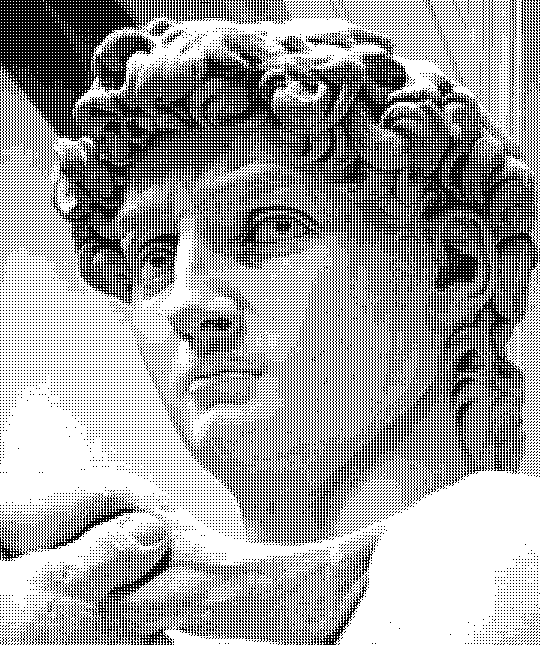
\includegraphics[scale=0.2]{figure/Ordered.png}
    }
    \caption{有序抖动的效果演示}
\end{figure}
有序抖动实际上是给图像添加了周期性的噪声后二值化的结果.例如,考虑抖动矩阵的元素$\mat{M}_{00}$,当$9g_{i}\geqslant6$,即$g_i-0.167\geqslant0.5$时,对应的像素点被设为黑色,也就是给该像素加上$-0.167$的噪声后进行二值化.我们将在下一节解释为何加上噪声后进行二值化可以得到更好的效果.
\subsubsection{基于噪声的抖动}
基于前面的思想,我们可以把图像加上随机生成的噪声后进行二值化.
\paragraph{噪声的作用}
我们假定原图第$i$个像素的灰度值为$f_i$,二值化后图像的第$i$个像素的灰度值为$g_i$.定义量化后图像与原图的平均误差$E$如下:
\[E=\dfrac{1}{N}\sum_{i=0}^{N-1}\left(f_i-g_i\right)\]
其中$N$为像素总数.我们希望$E$尽可能小.为此,考虑一种最简单的情形,令$f_i=0.25$.于是直接二值化的误差为
\[E=\dfrac{1}{N}\sum_{i=0}^{N-1}\left(\dfrac14-0\right)=\dfrac14\]
现在给每个像素加上均匀分布在$[-0.5,0.5]$的噪声$\ep_i$,然后再二值化.于是
\[E_{\text{noise}}=\dfrac{1}{N}\sum_{i=0}^{N-1}\left(\dfrac14-I_{0.25+\ep_i>0.5}\right)\]
其中$I_A$为事件$A$的示性函数,当$A$发生时取$1$,否则取$0$.由于$\ep_i$是一个随机变量,因此我们分析$E_{\text{noise}}$的数学期望:
\[\mathbb{E}\left(E_{\text{noise}}\right)
= \dfrac14-\dfrac{1}{N}\sum_{i=0}^{N}\mathbb{E}\left(I_{0.25+\ep_i>0.5}\right)
= \dfrac14-\dfrac{1}{N}\sum_{i=0}^{N}P\left(\ep_i>0.25\right)
= \dfrac14-\dfrac14=0\]
可以发现,在平均意义下加上噪声后二值化的误差变得更小.
\paragraph{白噪声与蓝噪声}
上述加噪声的办法(即给原像素加上均布于$[-0.5,0.5]$的噪声)称作\tbf{白噪声}.相比于直接二值化,白噪声抖动中的色带线性大大减轻,但仍然会出现明显的噪点.\\
\indent 改变噪声生成的方式,可以得到更好的效果.另一种常用的噪声是\tbf{蓝噪声}.典型的蓝噪声生成方式是在图像上随机生成一系列两两距离不小于某一值$r$的点,然后将该图像作为噪声的采样点进行二值化.
\begin{figure}[H]
    \centering\subfigure[源图像]{
        \includegraphics[scale=0.6]{figure/Origin.png}
    }\quad\quad
    \subfigure[经过白噪声处理后的图像]{
        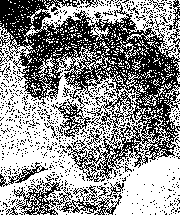
\includegraphics[scale=0.6]{figure/UniformRandom.png}
    }\quad\quad
    \subfigure[经过蓝噪声处理后的图像]{
        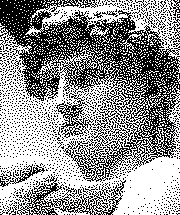
\includegraphics[scale=0.6]{figure/BlueNoise.png}
    }
    \caption{噪声抖动的效果演示}
\end{figure}
从频谱上看,白噪声的频谱是均匀分布的,而蓝噪声的频谱在低频部分较弱,在高频部分较强.由于人眼更难注意到高频信号,因此蓝噪声抖动后的图像看起来更为自然.
\subsubsection{基于误差扩散的抖动}
另一种抖动方法是\tbf{Floyd-Steinberg抖动算法}.它的基本思想是,在二值化某一像素后,计算该像素的量化误差,然后将该误差按一定权重分配给该像素周围尚未处理的像素.具体而言,我们从上到下,从左到右地处理图像的每一个像素.对于当前像素$i$,我们先将其灰度值$f_i$加上之前分配给它的误差$\ep_i$后进行二值化,得到二值化后的灰度值$g_i$.计算量化误差$\delta_i=f_i+\ep_i-g_i$,然后将$\delta_i$分为$7/16,5/16,3/16,1/16$四部分,分别加到它右边,左下,下方和右下的四个像素上.依次处理所有像素即可得到结果.
\begin{figure}[H]
    \centering\subfigure[源图像]{
        \includegraphics[scale=0.6]{figure/Origin.png}
    }\quad\quad
    \subfigure[误差扩散抖动处理后的图像]{
        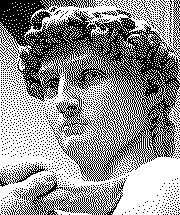
\includegraphics[scale=0.6]{figure/ErrorDiffuse.png}
    }
    \caption{误差扩散抖动的效果演示}
\end{figure}
这是一个确定性的算法,它的效果与噪声抖动相似,但不会出现明显的噪点或规则性斑点.然而,由于它需要逐像素处理并不断扩散误差,其计算速度相对更慢.
\end{document}